% ---------------------------------------------------------------------------
% Online Resource 5 -- Supplementary Information (four figures, text and tables)
%
% ONE file, assembled on 2026-10-06 from what used to be two:
%   supplementary_figures.tex      Fig. S1--S4        (was Online Resource 5)
%   supplementary_information.tex  sections S1--S24   (was Online Resource 6)
% The merge is why the main text now lists five online resources instead of six.
%
% Carries four figure plates (Fig. S1--S4) followed by the supporting detail the
% main text cites but does not develop, with Tables S5--S6 continuing the numbering
% of the four supplementary spreadsheets (Online Resources 1--4).
%
% The page geometry reproduces the published text block of the journal (174.9 mm
% wide, measured on a published article) rather than the narrower author template,
% so that a figure placed at \textwidth prints at the size it was drawn at and the
% type inside it keeps the point size declared in its generating script.
% ---------------------------------------------------------------------------
\documentclass[11pt]{article}

\usepackage[T1]{fontenc}
\usepackage[utf8]{inputenc}
\usepackage{newtxtext}
\usepackage{amsmath,amssymb}
\usepackage{graphicx}
\usepackage{booktabs}
\usepackage{multirow}
\usepackage[
  paperwidth=210mm,
  paperheight=279mm,
  left=17.55mm,
  right=17.55mm,
  top=22mm,
  bottom=22mm,
]{geometry}
\usepackage[round]{natbib}
\usepackage[hidelinks]{hyperref}

\setlength{\parindent}{0pt}
\setlength{\parskip}{2.5mm}

% Tables continue the supplementary numbering: S5, S6, ...
\renewcommand{\thetable}{S\arabic{table}}
\setcounter{table}{4}

\bibliographystyle{plainnat}

\begin{document}

\begin{center}
{\large\bfseries Supplementary Information}\\[2.5mm]
{\normalsize What is shared across 33 cancer types is the tissue, not the tumour: a non-malignant axis of the microenvironment}\\[1.5mm]
{\small Network Modeling Analysis in Health Informatics and Bioinformatics}\\[1.5mm]
{\small Shuaidong Gao}\\[0.8mm]
{\small Chongqing Institute of Foreign Studies, Qijiang Campus, Chongqing 401420, China}\\[0.8mm]
{\small Corresponding author: gaoshuaidong@stu.cqifs.edu.cn}
\end{center}

\vspace{4mm}

This file carries the four supplementary figures (Fig.~S1--S4) and the supporting
detail that the main text cites but does not develop: the synthetic validation of the two-stage framework (S1), the
hyperparameter grids behind the operating point (S2), the acyclicity
diagnostics (S3), the resampling, decomposition and stability analyses
(S4--S8), the robustness analyses of the recurrence result (S9--S15), the
extended limitations (S24), and Tables S5--S6. Sections, equations and tables
of the main text are referred to by name rather than by number. All numbers are
generated from the analysis outputs by scripts in the replication package.

\clearpage

\section*{Supplementary Figures}

{\setlength{\parskip}{0pt}%
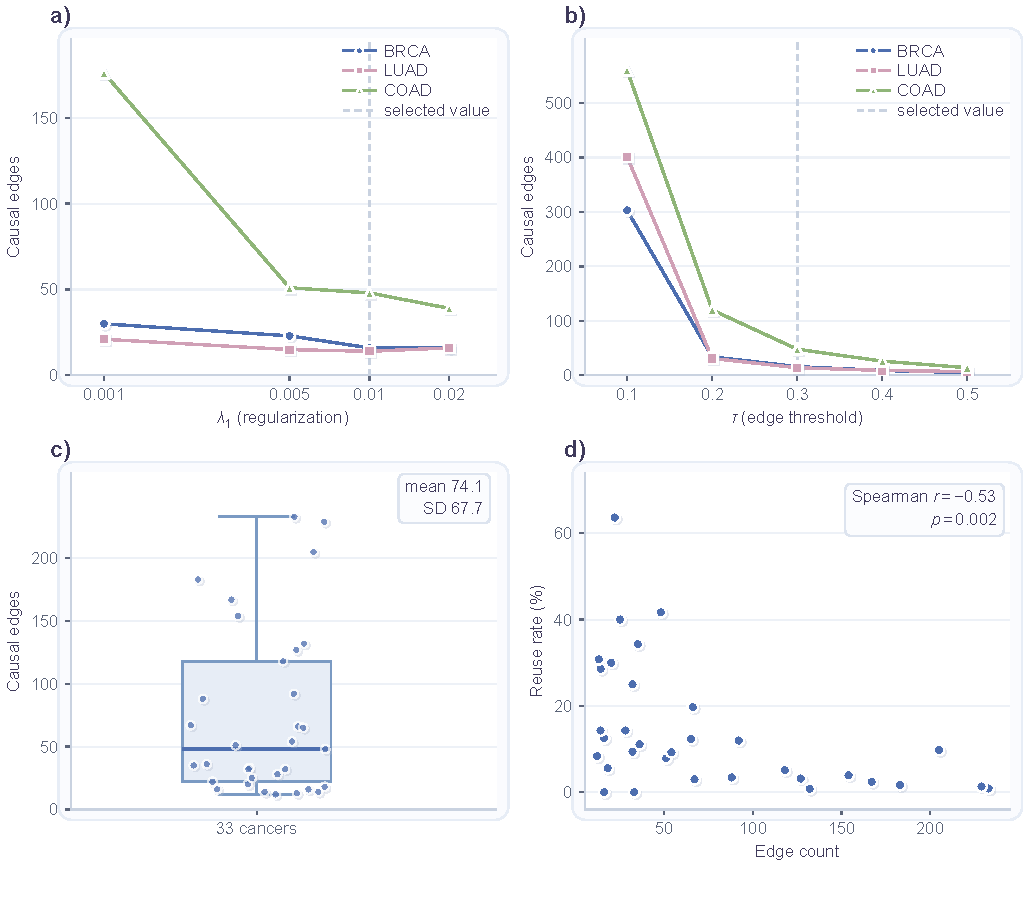
\includegraphics[width=\textwidth]{figures/FigS1.pdf}

\vspace{2.5mm}
{\small\textbf{Fig.~S1} Parameter sensitivity of the NOTEARS pipeline. \textbf{a)} $\ell_1$ regularization sensitivity for three representative cancers; $\lambda_1 = 0.01$ selected (dashed). \textbf{b)} Edge threshold $\tau$ sensitivity; $\tau = 0.3$ selected (dashed). \textbf{c)} Edge count distribution across 33 cancers (boxplot; mean 74.1, SD 67.7). \textbf{d)} Edge count vs per-cancer reuse rate (Spearman $r = -0.53$, $p = 0.002$)}
}

\clearpage

{\setlength{\parskip}{0pt}%
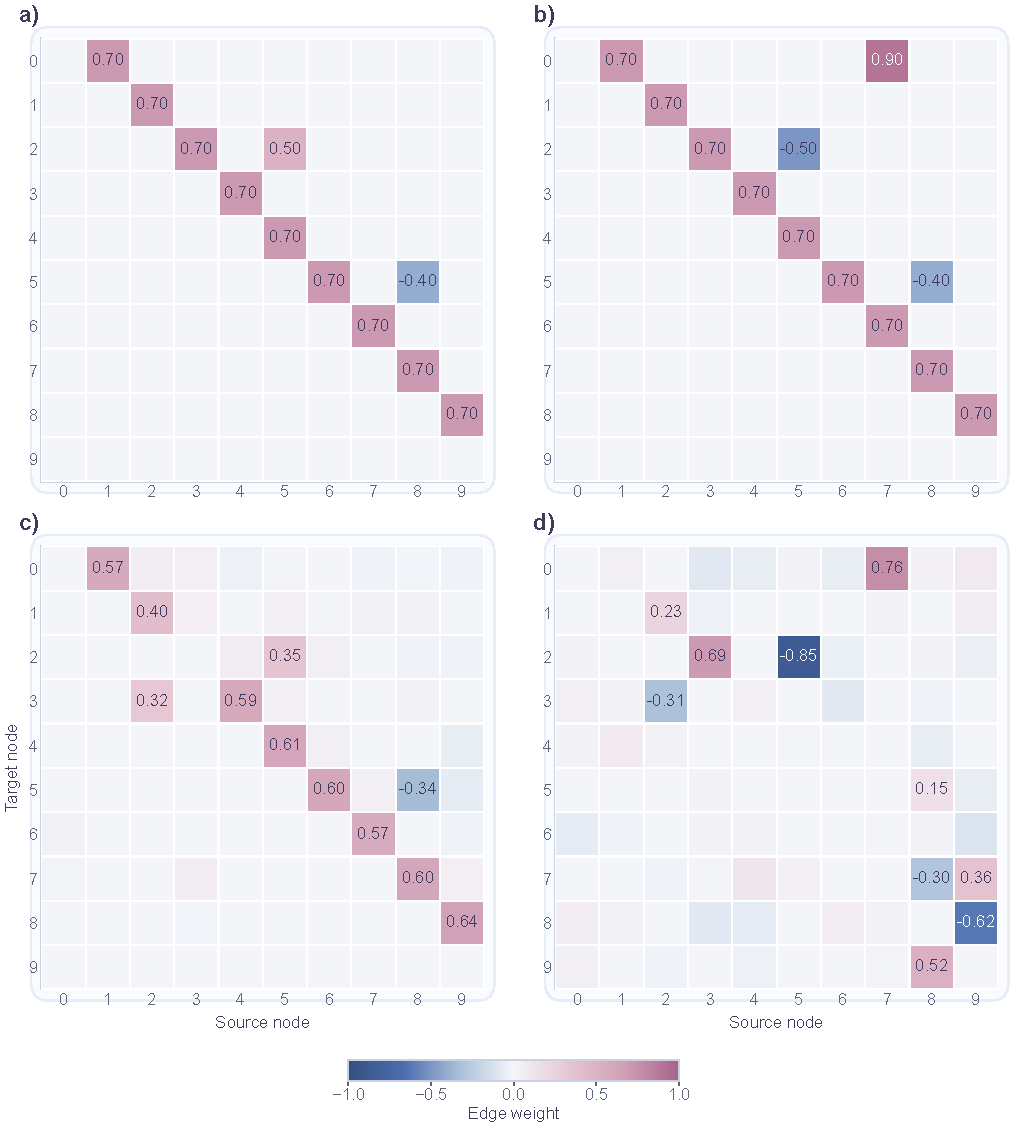
\includegraphics[width=\textwidth]{figures/FigS2.pdf}

\vspace{2.5mm}
{\small\textbf{Fig.~S2} Two-stage decomposition validation on a sparse chain-structured DAG ($d=10$, $K=3$). \textbf{a)} Ground truth shared backbone $W_0$ (11 edges). \textbf{b)} Ground truth Batch~1: rewired edge $2\to5$ (sign-flipped) and new edge $0\to7$. \textbf{c)} Recovered $\hat{W}_0$ from Stage~2 DAG projection (10/11 shared edges above $\tau=0.2$, $h(W_0)=5.21\times10^{-6}$). \textbf{d)} Deviation matrix $\Delta_1=\hat{W}_1-\hat{W}_0$ for the rewired batch. Overall recall: 14/15 ground-truth edges recovered ($=0.93$); the structure-recovery metrics are in Table~S5}
}

\clearpage

{\setlength{\parskip}{0pt}%
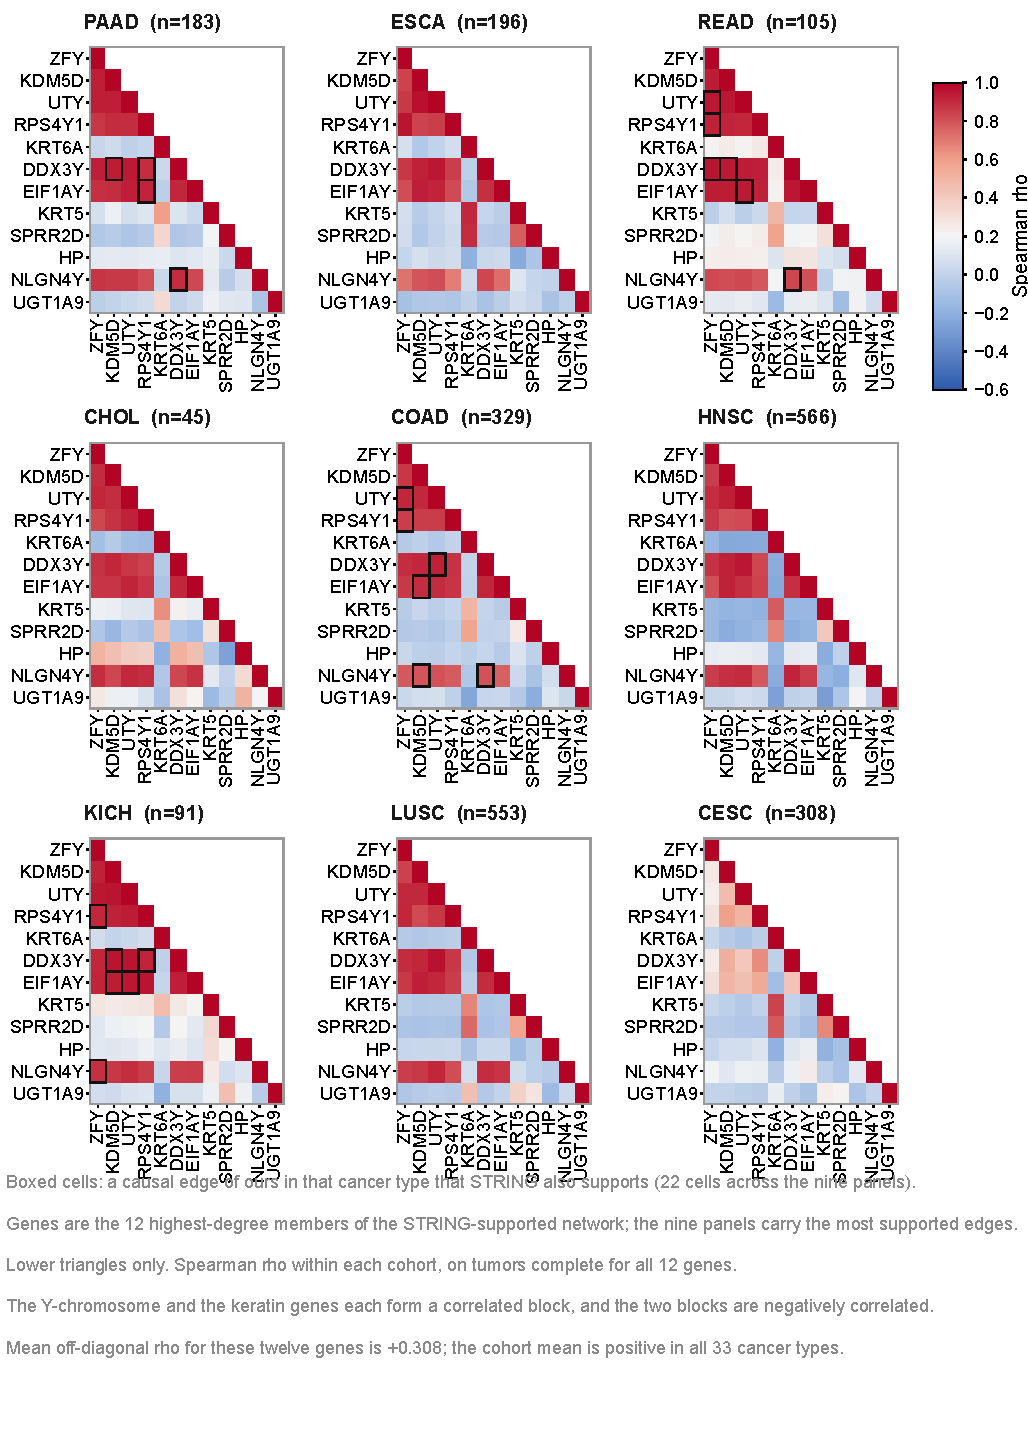
\includegraphics[width=\textwidth]{figures/FigS3.pdf}

\vspace{2.5mm}
{\small\textbf{Fig.~S3} Co-expression structure of the supported network. Lower triangles of the Spearman correlation matrix of the twelve highest-degree genes of the STRING-supported network, computed within each of the nine cohorts carrying the most supported edges. Boxed cells mark a causal edge of ours that STRING also supports. The Y-chromosome genes and the keratin genes each form a correlated block, and the two blocks are negatively correlated}
}

\clearpage

{\setlength{\parskip}{0pt}%
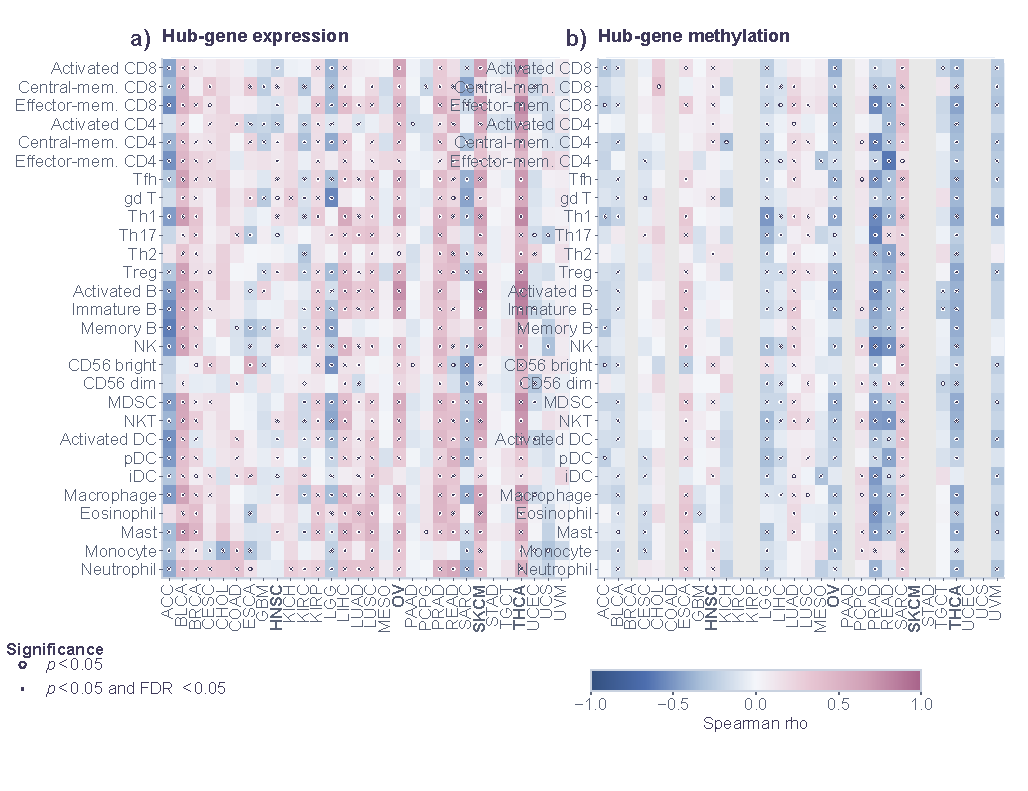
\includegraphics[width=\textwidth]{figures/FigS4.pdf}

\vspace{2.5mm}
{\small\textbf{Fig.~S4} Immune-microenvironment association of each cohort's own hub gene, with immune cell-type abundance taken from TISIDB (Ru et al., 2019). \textbf{a)} Hub-gene expression and \textbf{b)} hub-gene methylation against the abundance of the 28 TISIDB immune cell types, for the 30 cohorts carrying an immune profile; each cell is the Spearman $\rho$ between that cohort's own hub gene and that cell type, with significance marked as in the legend. Bold cohort labels mark hubs that are themselves immune-lineage markers; gray columns carry no data, methylation covering 21 cohorts. Expression is predominantly positive (306 of the 416 significant pairs) and methylation predominantly negative (175 of 270); the copy-number layer, with only 44 of 756 pairs significant, is not drawn. Excluding the four immune-lineage hubs, the hub still exceeds the other genes of its own network in 57.7\% of 728 pairs ($p = 4.4 \times 10^{-12}$), a modest effect (median $|\rho|$ 0.145 versus 0.122) that reverses in 10 of 26 cohorts}
}

\clearpage

\section*{Supplementary Text}

\section*{S1\ \ Synthetic validation}

We validated the framework on a sparse chain-structured DAG with $d=10$ nodes and $K=3$ batches. The shared DAG $W_0$ was a chain structure ($i \to i+1$ for $i=0,\dots,8$) augmented with two cross-edges ($2 \to 5$, $5 \to 8$). Batch~0 added two forward edges ($2 \to 6$, $4 \to 9$). Batch~1 added one ($0 \to 7$) and rewired $2 \to 5$ by flipping its sign relative to the shared backbone. Batch~2 was identical to $W_0$. Data were generated from linear structural equation models $X = \varepsilon (I - W_k)^{-1}$ with Gaussian noise ($\sigma = 0.02$, $n = 500$ per batch). The batches are fitted at their generated scale---no standardisation is applied to the synthetic data, so $\sigma = 0.02$ is the noise scale the estimator sees and the edge weights are compared to ground truth on the same scale; the TCGA matrices, by contrast, are standardised column-wise before fitting (the Data subsection of the main text). The benchmark is deliberately small and low-noise---$d = 10$ nodes at $\sigma = 0.02$---so it establishes that the two-stage pipeline recovers a known shared backbone and separates it from batch-specific edges under controlled conditions; it is not evidence that the same recovery holds at $d = 100$ under real expression noise, which the TCGA analysis tests directly rather than by analogy.

On the $d=10$, $K=3$ synthetic benchmark (Fig.~S2), Stage~1 NOTEARS recovered 13, 13, and 11 edges for the three batches (ground truth: 13, 12, and 11, respectively). The elementwise median produced an initial shared estimate $\bar{W}$ with 11 edges and DAG constraint violation $h(\bar{W}) = 1.1 \times 10^{-3}$. After Stage~2 DAG projection, the refined shared backbone $W_0$ achieved $h(W_0) = 5.2 \times 10^{-6}$, an improvement by a factor of about 200, while preserving 10 of 11 shared edges. All four batch-specific edges were accurately recovered in the corresponding $\Delta_k$ matrices, with estimated weights deviating from ground truth by an average of 16\%. Overall, 14 of the 15 ground-truth edges were recovered (recall $= 0.93$), consistent with the structure-recovery metrics reported below (Table~\ref{tab:synth_metrics}). The framework correctly distinguishes shared structure from context-specific regulation, including the rewired edge in Batch~1 whose sign flip was accurately detected in $\Delta_1$. \textbf{The framework is validated in its design regime, a common panel across batches; the complementary regime, in which each cohort carries its own gene set, is handled by the gene-pair layer of the main text.}

To align with standard evaluation practice, we additionally report the conventional structure-recovery metrics (Precision, Recall, F1, FDR, and directed SHD) computed directly against the known synthetic ground-truth DAG in addition to raw edge counts (Table~\ref{tab:synth_metrics}). In the $\tau=0.2$ operating point adopted for the synthetic benchmark (distinct from the $\tau=0.3$ used for TCGA in Parameter sensitivity in the main text), we observe two complementary findings. First, the Stage-2 projected shared backbone $W_0$ reproduces 10 of the 11 shared edges and introduces no edge outside the ground-truth skeleton, but returns one of them in the reverse orientation (ground-truth weight $0.7$, recovered as $0.32$ in the opposite direction), giving Precision $=$ Recall $=0.91$, F1 $=0.91$, FDR $=0.09$, and directed SHD $=3$. The DAG projection nonetheless removes every spurious edge that Stage-1 NOTEARS introduces at small sample size: Batches~0 and~1 each carry three false positives before projection (FDR $=0.23$) and none in the projected backbone outside the skeleton, so it remains the deferred-cleaning step that yields a clean shared skeleton.

Second, the end-to-end per-batch reconstruction, which retains Stage-1 estimation noise, achieves F1 $=0.77$--$1.00$ and FDR $=0.00$--$0.23$, with Batch~2 (exactly matching the shared backbone) recovered perfectly (Precision $=$ Recall $=$ F1 $=1.00$, SHD $=0$). All four batch-specific edges (two in each of Batch~0 and Batch~1), including the sign-flipped rewired edge in Batch~1, are recovered, while the single shared edge returned with reversed orientation (an inner chain edge, ground-truth weight $0.7$) appears in the opposite direction. The residual false positives in Batch~0 and Batch~1 arise from the small per-batch sample ($n_k = 500$, $d=10$), not from the decomposition procedure itself; these metrics are stable across the threshold grid ($\tau \in [0.1, 0.3]$): the projected backbone returns the same Precision, Recall, F1, FDR, and SHD at every threshold tested.

\begin{table}[htbp]
\centering
\caption{Standard structure-recovery metrics on the synthetic benchmark ($d=10$, $K=3$) at $\tau=0.2$. Precision, Recall, F1, and FDR follow the standard definitions against the ground-truth DAG; SHD is the directed structural Hamming distance (symmetric difference plus reversed edges). The Stage-2 projection recovers 10 of the 11 shared edges and introduces no edge outside the skeleton, but returns one shared edge with its direction reversed; the end-to-end Stage-1 reconstruction retains a larger amount of false-positive noise at small sample size}
\label{tab:synth_metrics}
\begin{tabular}{lcccccc}
\toprule
Target & Precision & Recall & F1 & FDR & SHD \\
\midrule
Stage-2 shared backbone $W_0$ & 0.91 & 0.91 & 0.91 & 0.09 & 3 \\
End-to-end Batch 0 & 0.77 & 0.77 & 0.77 & 0.23 & 8 \\
End-to-end Batch 1 & 0.77 & 0.83 & 0.80 & 0.23 & 6 \\
End-to-end Batch 2 & 1.00 & 1.00 & 1.00 & 0.00 & 0 \\
\midrule
\multicolumn{6}{l}{\small Ground truth: shared backbone 11 edges; batch-specific 4 edges.}\\
\bottomrule
\end{tabular}
\end{table}

\section*{S2\ \ Parameter sensitivity and robustness}

The NOTEARS objective exposes two hyperparameters that affect edge recovery: the $\ell_1$ regularisation strength $\lambda_1$, and the edge detection threshold $\tau$. We conducted a sensitivity analysis on three representative cancers that span the sample-size range of the panel (BRCA, 1{,}218 tumours; LUAD, 576; COAD, 329; Fig.~S1). For $\lambda_1 \in \{0.001, 0.005, 0.01, 0.02\}$, per-cancer edge counts at each value were (BRCA: 30, 23, 16, 16; LUAD: 21, 15, 14, 16; COAD: 176, 51, 48, 39). The COAD count at $\lambda_1 = 0.001$ stands out in the grid---more than three times that cohort's next value and an order of magnitude above the other two cohorts---and has the profile of an under-regularised fit rather than of biology, which is one reason the operating point sits well above it. We selected $\lambda_1 = 0.01$ as the operating point because edge counts had stabilised by that value in all three cohorts while the recovered networks stayed compact, and because the augmented Lagrangian behaved stably across the grid. Hyperparameter choice is a recognised source of variability in structure learning: a systematic study found that algorithms differ more from one another in their sensitivity to hyperparameters than any one algorithm differs across datasets \citep{machlanski2024robustness}. The full grid is reported here alongside the selected operating point.

For the edge detection threshold $\tau$, we examined $\tau \in \{0.1, 0.2, 0.3, 0.4, 0.5\}$; per-cancer edge counts were (BRCA: 303, 34, 16, 9, 5; LUAD: 401, 31, 14, 9, 7; COAD: 560, 120, 48, 26, 14). At $\tau = 0.1$, edge counts were inflated (median 401 across the three cohorts), driven by estimation noise. At $\tau = 0.5$, edge counts collapsed (median 7), retaining only the strongest edges. $\tau = 0.3$ provided a balanced operating point (median 16 edges), and we adopt it throughout. Because a continuous-optimisation solution is threshold-free, the value of $\tau$ is a reporting choice, stated explicitly so that the edge counts above can be reproduced~\citep{zheng2018dags}. All subsequent analyses use $\lambda_1 = 0.01$, $\tau = 0.3$ for TCGA data.

\section*{S3\ \ Acyclicity at the operating point}

\subsection{Acyclicity at the operating point}
\label{si:acyclic}

The acyclicity NOTEARS imposes is a property of the optimisation rather than of the thresholded graph, so we state how far it holds in practice. The augmented Lagrangian is capped at 100 outer iterations, each an L-BFGS-B subproblem capped at 200 iterations, and stops early once $|h(W)| < 10^{-7}$; none of the 33 cohorts reached that tolerance. The iterate returned is the least-violating one seen, with $|h(W)|$ between $1.1 \times 10^{-3}$ and $1.8 \times 10^{-1}$ (median $4.4 \times 10^{-2}$); four cohorts fall below $10^{-2}$ and six exceed $10^{-1}$ (OV, LUAD, SARC, SKCM, PRAD and KIRC). The fitted matrices are therefore near-acyclic instead of exactly acyclic, and the graphs analysed below are the entries that survive thresholding at $\tau = 0.3$, not the raw optimiser output.

Thresholding removes most of what remains. Sixteen of the 33 thresholded graphs are acyclic; in the other 17, the 109 edges that lie on a directed cycle amount to 4.5\% of the 2,445 edges. Three of the six cohorts above $10^{-1}$ (OV, PRAD, KIRC) are acyclic once thresholded, and the other three carry 13 of those 109 cyclic edges between them. No pair is reciprocated within a single cohort's graph, so every cycle has length three
or more, and the cyclic edges concentrate in the sex-chromosome and paralogue clusters (the
recurrent pairs of those two classes are tabulated in Online Resource~3). The recurrence
result of the recurrence analysis in the main text does not depend on them: none of the 14 recurring pairs of
the aligned panel lies on a directed cycle in any cohort, and of the 19 shared pairs of the
per-cohort design the nine that do are all sex-chromosome pairs (XIST--TSIX and the
Y-chromosome cluster).
Reciprocity does appear once the cohorts are pooled, and is reported in
the recurrence analysis in the main text. That concentration is consistent with the interpretation in the sample-size analysis in the main text: these edges arise from under-determined fitting. The per-cohort violation and a flag on every cyclic edge are written to the replication package (\texttt{\_acyclicity.json}).

\section*{S4\ \ How far the orientations survive resampling}

The comparison above is element-wise, so every recurring pair arrives with an orientation, and the orientation is the part of a NOTEARS output that observational Gaussian data do not identify: with equal residual variances the likelihood of an edge is the same in either direction, and the score is broken only by acyclicity and by the numerics of the optimiser. We therefore ask how far each orientation survives resampling instead of reading the arrows as findings.

Two resampling schemes were run on the aligned panel. In the first, each cohort's samples were drawn with replacement ($B = 6$ draws per cohort) and the graph refitted; for each of the 14 recurring pairs we then restricted attention to the cohorts whose original fit placed that directed edge and counted the resamples in which the edge reappeared above $\tau$ with the same sign. Retention ranges from $0.67$ (IGJ$\rightarrow$MZB1, 60 draws over ten supporting cohorts) to $0.88$ (HBB$\rightarrow$HBA1, 138 draws over 23), with a mean of $0.77$ across the 14 pairs; the two chemokine pairs retain at $0.86$ and $0.78$. No resample produced the reverse edge --- whenever a directed edge reappeared it carried its original sign, so skeleton and orientation retention coincide exactly for all 14 pairs, and what resampling removes is the edge rather than its direction.

In the second scheme each cohort was refitted from six random initialisations with the data held fixed, over the 20 cohorts that yield the most edges. Agreement with the original orientation is much lower here: it averages $0.49$ across the pairs and ranges from $0.28$ (IGJ$\rightarrow$MZB1) to $0.76$ (CXCL10$\rightarrow$CXCL11). The two schemes perturb different things: resampling changes the sample while leaving the optimiser's path intact, whereas re-initialisation changes the path on the same likelihood surface. The lower agreement is therefore the relevant figure for a reader asking whether an independent run would recover the direction.

Both schemes are finite-sample statements. The bootstrap covers all 33 cohorts, drawing on between 60 and 168 refits per pair, so its agreement for a single pair is resolved to a binomial standard error of at most $(0.25/n)^{1/2} = 0.065$; the re-initialisation covers the 20 densest cohorts at a fixed six restarts each, so every pair has $n = 120$ and a standard error of at most $0.046$. Narrower intervals at a larger draw count would not move either mean, so the qualitative reading these two schemes were run to establish---independent restarts agree with the original orientation for about half the pairs, sample resampling for about three quarters---is a statement about the level of agreement rather than about the third decimal of any one pair.

The consequence for reading the recurrence table of the main text is that the ``Cohorts'' column is a statement about an edge being present at a directed position, and the ``Basis'' column is where the direction is adjudicated. Two pairs are supported by both schemes and by a known mechanism: CXCL9, CXCL10 and CXCL11 are co-induced as a set by interferon-$\gamma$~\citep{groom2011cxcr3,metzemaekers2017nonredundant}, their retention is the highest of the 14 under both schemes, and the direction attached to them is best read as an ordering imposed on a relation that the data make symmetric. For the pairs marked \emph{both} the two orientations are within a few cohorts of each other, so nothing prefers one. For the remaining pairs the arrow should be read as the estimator's ordering of a dependence it detects reliably, which is the same conclusion the composition-adjusted refit in the main text reaches from a third direction: a composition-adjusted refit lowers the orientation agreement of exactly the pairs already flagged as two-sided.

\section*{S5\ \ The two-stage decomposition on the aligned panel}

The framework of the aligned-panel subsection of the main text was validated on synthetic data (Synthetic validation in the main text); running its second stage (\ref{eq:stage2}) on the 33 aligned cohorts is informative about the recurring set itself, because it separates what all cohorts share from what only some do. The elementwise median $\bar{W}$ is already almost acyclic, with $h(\bar{W}) = 4.5 \times 10^{-3}$, and every one of the 33 individual fits has a larger violation (per-cohort $h$: minimum $1.2 \times 10^{-2}$, median $8.6 \times 10^{-2}$, maximum $1.4 \times 10^{-1}$) --- so the DAG constraint is imported at a cost that the shared estimate, unlike a single cohort, has nearly paid already. Projecting at $\lambda_{\mathrm{proj}} = 0.001$ leaves the thresholded edge set unchanged: six edges above $\tau$ at exactly the same positions, weights essentially untouched (largest $|\bar{W}_{ij}|$ $0.731$ before and $0.730$ after), and six of the 14 recurring pairs inside the projected backbone. The projection's constraint violation reaches $5.2 \times 10^{-7}$ under the textbook augmented-Lagrangian schedule, which escalates the penalty while $h$ exceeds tolerance, but only $4.2 \times 10^{-3}$ under the schedule the synthetic benchmark uses, which escalates only when $h$ increases; we report both because the difference is what tells a reader whether the projection is a small correction or an unconverged one. The edge set is identical either way. On this dataset the projection therefore confirms that the shared estimate is already essentially acyclic rather than altering the result; what the stage adds is the separation of $W_0$ from $\Delta_k$ reported next, and the demonstration that it cleans an estimate with a large acyclicity violation is carried by the synthetic benchmark, where it removes every spurious edge Stage~1 introduces (Synthetic validation in the main text).

What the decomposition mainly establishes is how thin the shared backbone is relative to any single cohort. Averaged over the 33 cohorts, $84.6\%$ of a cohort's $\tau$-level edges are absent from the shared backbone (range $58.3$--$99.1\%$), about 64 cohort-specific edges per cohort, and the Frobenius norm of the deviation $\Delta_k$ averages $5.9$. The deviation matrices are dense at the $0.01$ soft-threshold the framework specifies for suppressing estimation noise, because NOTEARS returns many coefficients below the edge threshold, which is why we report them at the $\tau$ scale: the interpretable quantity is the share of a cohort's edges the backbone does not contain. The recurring set is therefore the small part of each graph that survives across cohorts, not a compressed description of it --- the quantitative form of the claim that what reproduces is the axis rather than the edge.

\section*{S6\ \ The boundary is measured at each width}

If the floor were a property of the estimator rather than a measurement on this dataset, the boundary would keep a fixed ratio to the panel width. We repeated the shuffle control at four widths on the same top-$d$ dispersion panels, so that the ratio can be read off rather than extrapolated. It is not fixed. The smallest cohort that returns no edges on shuffled data sits at $n^{*} = 80$ for $d = 50$ ($1.60d$), $156$ for $d = 100$ ($1.56d$), $173$ for $d = 150$ ($1.15d$) and $187$ for $d = 200$ ($0.94d$). At $d = 200$ a cohort at $n = 196$ still generates edges while one at $n = 187$ does not, so the two regimes overlap and the boundary is no longer sharp.

The scan supports two stable findings. At every width the largest cohort still generating edges on shuffled labels lies at or below $1.6d$. And at every width the shuffled data reproduce the dependence of edge count on sample size that the real data show: the real correlation strengthens with width ($r = -0.50$, $-0.65$, $-0.71$, $-0.74$ at $d = 50$, $100$, $150$, $200$) and the shuffled control tracks it ($-0.33$, $-0.52$, $-0.55$, $-0.59$ at the same widths). The dependence is thus a property of the fitting problem at every width, while the position of the boundary is not, and we do not import a constant for it. What the scan establishes is that the floor has to be located on the study's own data, which the shuffle does in a single pass, and that a margin stated as a multiple of $d$ is only as good as the width at which it was measured. Two independent realisations at $d = 100$ bracket the boundary within a single cohort width---one separates the regimes between $n = 122$ and $n = 156$, the other between $n = 156$ and $n = 172$---so that even at one width the figure moves with the draw and is better reported as a range than as a value.

\section*{S7\ \ The recurring pairs carry no copy-number coupling}

The attribution developed above reads the recurring set on the expression axis, so the one genomic layer that can produce correlated expression between two genes with no regulatory relation between them has to be separated from it: somatic copy number. The aligned-panel diagnostics already drew on the GISTIC~2 thresholded matrix, but as a cross-platform check on the dominant principal component rather than on the 14 pairs themselves (the aligned-panel subsection of the main text). We therefore measured the pairs directly. Thresholded copy-number states were taken from the pan-cancer GISTIC~2 matrix distributed through UCSC Xena \citep{goldman2020visualizing} (10{,}845 samples over the 33 cohorts), of which 9{,}415 belong to the cohorts analysed here, and the two genes of each pair were correlated over those samples. Because copy number is spatially organised, a null is required rather than optional: 2{,}000 random gene pairs were drawn in five genomic-distance strata of 400 each from a fixed set of 1{,}055 genes, and every recurring pair was placed inside the stratum its own separation defines.

Copy-number co-variation falls monotonically with distance---median Spearman $\rho$ of $0.980$ within 1~Mb, $0.902$ between 1 and 10~Mb, $0.606$ between 10 and 100~Mb, $0.104$ beyond 100~Mb on the same chromosome and $0.042$ across chromosomes (Fig.~8 of the main textb)---so a correlation near unity is the expected behaviour of neighbouring genes rather than evidence of anything. All 14 pairs sit below the 95th percentile of their own stratum. The set nevertheless separates in two at the genomic scale (Fig.~8 of the main texta). The five cis pairs lie 13--462~kb apart and correlate at $\rho = 0.98$--$1.00$, inside the neighbouring-gene background; that includes CXCL9--CXCL10 and CXCL10--CXCL11, which sit 13--18~kb apart in the 4q21.1 chemokine cluster, one of the most familiar co-amplified regions in cancer genomics. Physical proximity alone cannot exclude co-amplification for those pairs, so it was tested rather than assumed. The nine trans pairs behave differently: they join genes on different chromosomes, correlate at $\rho = -0.03$ to $0.13$, and are indistinguishable from the cross-chromosome background (Mann--Whitney $p = 0.105$), while the two classes differ from each other ($p = 0.0016$). No copy-number mechanism links genes on different chromosomes at this resolution, so the recurrence of those nine is left to the abundance reading that the composition-adjusted refit in the main text reaches independently. The recurring set is therefore scale-dependent in what can be claimed for it, and the recurrence table of the main text carries that limit as a column rather than in prose alone.

Testing the cis pairs means asking whether their co-expression survives removal of copy number. For each of the four cis pairs---five cis edges, since CXCL1/CXCL8 is recovered in both orientations---each gene's expression rank was residualised on that gene's own thresholded copy-number state within a cohort, and the correlation recomputed on the residuals. The correlation is essentially untouched, so copy number carries none of the coupling: CXCL10--CXCL11 at a median $\rho$ of $0.911$ before and $0.911$ after, CXCL9--CXCL10 at $0.853$ and $0.853$, CXCL1--CXCL8 at $0.724$ and $0.721$, and C7--PLCXD3 at $0.624$ and $0.627$. The adjusted correlation stays at or above $0.30$ in 33, 33, 31 and 29 of the 33 cohorts respectively. Two direct checks agree. The 4q21.1 locus is gained in only 8.6\% of the analysed samples, so an account that made co-amplification responsible would have to generate a recurrence in 26--28 cohorts from a variant carried by fewer than a tenth of them; and in DLBC, where the locus is not gained at all, the pair still co-varies at $\rho = 0.941$, while in ACC, where 39.0\% of samples carry the gain, residualising moves the correlation by $0.001$. The cis pairs therefore enter the recurrence table of the main text as a statement of what copy number cannot be excluded from by distance alone, not as a mechanism the data support.

\section*{S8\ \ Controlling for tissue composition}

If the recurring pairs were a restatement of ``this sample contains more non-malignant tissue'', then removing a measurement of non-malignant content from every panel gene should dissolve them. We tested this directly: each sample was scored on the same 22 immune, stromal and endothelial markers drawn from outside the panel, every one of the 100 panel genes was residualised on that score, and all 33 cohorts were refitted --- so the composition axis is removed from the data before the estimator sees it, rather than regressed out of the answer afterwards.

The shared structure survives. Thirteen of the 14 recurring pairs still recur in ten or more cohorts, the shared median matrix has seven edges above $\tau$ against six before, and its largest coefficient is $0.732$ against $0.731$. Pair by pair, the raw and composition-adjusted associations are close: the chemokine pairs lose little (CXCL9$\rightarrow$CXCL10 mean $r$ $0.839 \rightarrow 0.779$; CXCL10$\rightarrow$CXCL11 $0.898 \rightarrow 0.870$) and the blood-content and immunoglobulin pairs almost nothing (HBB$\rightarrow$HBA1 $0.804 \rightarrow 0.799$; ADAM6$\rightarrow$IGJ $0.889 \rightarrow 0.834$). What the adjustment does change is the orientation balance of the pairs already flagged as two-sided in the recurrence table of the main text. The neutrophil pair becomes symmetric (CXCL1$\rightarrow$CXCL8 in 18 cohorts against the reverse in 14, from 33 against 0), as does the plasma-cell pair (ADAM6$\rightarrow$IGJ 17 against the reverse 14), and the haemoglobin pair loses its leading orientation (HBA1$\rightarrow$HBB clears $\tau$ in 8 cohorts against 25 for the reverse, having been 10 against 23). The chemokine pairs keep their one-sidedness throughout (CXCL10$\rightarrow$CXCL11 29 cohorts against 3; CXCL9$\rightarrow$CXCL10 27 against 1). The adjustment therefore removes a direction, not a pair.

We read this as bounding a confound, not as eliminating it. The adjustment removes one composite axis built from 22 markers, and it cannot separate composition from biology as cleanly as deconvolution with cell-type-specific expression would: an unmeasured component of the mixture, and any marker that is itself co-regulated with the panel genes, stays in the residual. What the test does establish is that the recurrence is not mediated by the bulk-content axis that the panel's own first component measures --- the specific mechanism by which a dispersion-selected panel could have manufactured it --- and it is one of the two falsification conditions stated in the Discussion.

\section*{S9\ \ Length-two path enumeration and the threshold dependence of the count}

On the aligned panel the 33 cohorts contribute 2{,}239 edges over the 9{,}900 directed gene pairs the panel admits. Recurrence is rare and unevenly distributed. Fourteen pairs---0.14\% of the space---are recovered in ten or more cohorts (Fig.~1 of the main text; the recurrence table of the main text). The count is significant against the gene-wise permutation null but not against covariance-matched nulls in count, so what singles this set out is its composition rather than its size (the null-panel analysis in the main text); the most prominent member is a single three-gene module rather than a scattered set. CXCL9--CXCL10 is recovered in 26 of 33 cohorts and CXCL10--CXCL11 in 28 of 33, and the three chemokines form one connected component rather than three unrelated edges. We do not read that component as a directed cascade, because the known regulation is parallel rather than sequential. CXCL9, CXCL10 and CXCL11 are the three interferon-$\gamma$-inducible ligands of CXCR3, and reviews of the system conclude that they act in a non-redundant, ligand-specific manner rather than as interchangeable members of one chain, recording claims of ``mutual redundancy, ligand dominance, collaboration or even antagonism'' that depend on context~\citep{metzemaekers2017nonredundant}. Groom and Luster make the same point in the form that matters here---some studies report that the ligands have ``redundant functions in vivo'', others that they ``can also collaborate and even compete with each other''---and the ligands are not even induced together, since CXCL10 also responds to innate type~I interferon whereas CXCL9 induction is restricted to interferon-$\gamma$~\citep{groom2011cxcr3}. No evidence establishes that CXCL9 regulates CXCL10 or that CXCL10 regulates CXCL11. The arrows the estimator places on these two edges are therefore the orientation it selected, not a direction the data identify, and the orientation-resampling analysis in the main text quantifies how far that orientation survives resampling.

Every other recurring pair sits on the same kind of axis: interferon-$\gamma$/CXCR3 chemokines (CXCL9, CXCL10, CXCL11), neutrophil/CXCR2 chemokines (CXCL1, CXCL8), blood content (HBA1, HBB), possibly including haemolysis (Limitations of the main text), the plasma-cell immunoglobulin locus (ADAM6, IGJ, MZB1), stromal abundance (COL10A1, COL11A1, C7, and PLCXD3, which remains poorly characterised and to which we attach no mechanistic claim), and myeloid/macrophage abundance (IL6, FOSB, CCL18, CHIT1). Symbols follow current HGNC nomenclature; where the source matrices carry a legacy spelling, it is replaced by the current symbol in the text, the tables and the figures (IL8 for CXCL8). None of the 14 involves a canonical driver gene.

The three-gene module is also the only length-two path of its kind in the set, a claim we
make explicit so that it can be verified. We define a length-two path as
$A \rightarrow B \rightarrow C$ whose two edges are each recovered in ten or more cohorts
and neither of which is recovered in the reverse orientation, so that both edges keep a
single estimated direction across cohorts. Eight of the 14 recurring pairs meet that
requirement (the recurrence table of the main text; the qualification is stated below). Exactly one pair of
those eight shares its middle node, and it is CXCL9$\rightarrow$CXCL10$\rightarrow$CXCL11.
If the requirement is relaxed to admit the three reciprocated pairs, two further
length-two paths appear---ADAM6$\rightarrow$IGJ$\rightarrow$MZB1 and
IGJ$\rightarrow$ADAM6$\rightarrow$MZB1---but both run through a reciprocated edge. The
enumeration is stated in full so that the count can be verified.

The recurrence rate is far above what the panel geometry would generate by itself. Under the 500 permutations described in the aligned-panel subsection of the main text, no pair reaches ten cohorts (observed 14, maximum under the null 0), the count at five cohorts falls from 34 to a null mean of 0.02, and the collision statistic---the sum over pairs of the squared recurrence count---drops from 8{,}037 to 2{,}715 $\pm$ 32, giving $z = 166.8$ ($p \leq 0.002$). That permutation removes every between-gene dependence within a cohort, so it establishes only that the recurrence is not an artefact of the panel geometry or of the number of edges fitted; the stronger test, against nulls that retain each cohort's covariance structure and destroy only the cross-cohort correspondence of edges, is reported in the null-panel analysis in the main text.

The same table supports three qualifications, carried through the rest of the paper. First, of the 14 edges three are recovered in both orientations (ADAM6$\leftrightarrow$IGJ, CXCL1$\leftrightarrow$CXCL8, HBA1$\leftrightarrow$HBB), so only eight carry an unambiguous direction. Second, the permutation test shows that the recurrence is not expected under exchangeability, but it does not license a causal reading of any individual edge. We therefore describe the recurring set as conditional dependencies at the transcript level throughout. Third, correlated expression can be produced without any regulatory relation when two genes share a copy-number state, and no check reported so far rules that out for these particular pairs; the one genomic layer that can manufacture the whole recurring set is measured directly in the copy-number analysis in the main text and entered in the ``CN $\rho$'' column of the recurrence table of the main text.

The count itself is threshold-dependent, because $\tau$ is the reporting threshold rather than a fitted parameter. Recomputing the recurrence from the stored aligned-panel matrices, with no refitting, gives $44$ pairs at $\tau = 0.15$, $27$ at $0.20$, $17$ at $0.25$, $14$ at $0.30$, $12$ at both $0.35$ and $0.40$, $10$ at $0.45$ and $7$ at $0.50$ (Table~\ref{tab:tau}). The number of recurring pairs is therefore a property of the threshold as much as of the tumours, which is a further reason to read recurrence as evidence for the \emph{axis} rather than for the count. What does not move is the chemokine module: CXCL9$\rightarrow$CXCL10 and CXCL10$\rightarrow$CXCL11 stay above ten cohorts across the whole range, at $21$--$28$ and $28$--$29$ of the 33 cohorts.

\section*{S10\ \ Null panels that preserve the selection regime}

The permutation check of the sample-size analysis in the main text destroys all between-gene dependence within a cohort, so it answers only whether recurrence is an artefact of the panel's geometry. A harder question is whether a panel assembled by the same rule from unrelated genes would reproduce the same structure, which is the null a reader worried about selection needs. We built four such nulls and refitted all 33 cohorts on each.

The two that destroy gene identity return nothing. Rotating each cohort's panel by an independent random orthogonal matrix preserves the eigenvalue spectrum of that cohort's covariance matrix exactly---and therefore its total variance---while making every resulting variable a mixture of the 100 genes, so that no variable retains a gene's identity, and across three realisations the median matrix holds no entry above $\tau$ and no pair reaches ten cohorts; permuting sample labels within each gene does the same, which is the result reported above.

The two that preserve the selection regime do return structure, which is the informative outcome. Twelve replacement panels were drawn by exchanging each panel gene for a gene outside the panel from the same decile of mean expression, and twelve more matched on the deciles of mean expression \emph{and} of across-cohort median MAD, so that the second family is selected exactly as the real panel is. The expression-matched family is quiet: its median matrix holds $0$--$4$ entries above $\tau$ against $6$ for the real panel, its largest median coefficient is at most $0.538$ against $0.731$, and its recurring pairs number $2$--$11$ (mean $6.4$). The double-matched family is not quiet: median-matrix density rises to $2$--$5$, the largest median coefficient to $0.638$, and the recurring count to $6$--$15$ (mean $9.8$), which brackets the real panel's fourteen. A third family, drawn from the low-dispersion half of the distribution, falls to $0$ entries, one recurring pair and a largest median coefficient of $0.237$.

The families together separate two quantities that the count alone conflates. Density and coefficient strength do discriminate: the real panel's median matrix carries six entries above $\tau$ and a largest median coefficient of $0.731$, and none of the twenty-four constructed panels reaches either (best $5$ and $0.638$; the real panel ranks first of the twenty-five panels compared, which is the best rank this number of panels admits and is reported as a descriptive rank rather than as a calibrated $p$-value), while the recurring \emph{count} does not ($14$ against a maximum of $15$, and a mean of $9.8$ in the matched family). What the matched families recover is again an axis rather than a pair, and it is a different axis: their recurring pairs are dominated by a tandem duplicate on $10p15$---AKR1C1--AKR1C2 in twelve and eleven of the twelve double-matched panels---and by the interferon-inducible GBP5, and in the expression-matched family not one of the $77$ recurring pairs appears in two of the twelve panels. The chemokine genes cannot appear in a replacement panel at all, since the pool is drawn from outside the real panel, so their absence carries no information; what the nulls do show is that the strongest recurring set any of them reaches is the AKR1C1--AKR1C2 tandem duplicate rather than a co-induced three-gene module of the kind the chemokine triplet represents. Selection on dispersion therefore enlarges the recurring set, which is why we report the count with its null and do not use it as evidence, but it does not manufacture the module. That is identified instead by its convergence with STRING, its correlation with panel-exogenous markers, and its survival under composition adjustment---none of which the constructed panels reproduce.

\section*{S11\ \ Panel independence of the axis and the sample-size dependence}

The number of edges a cohort yields is strongly tied to its sample size, and the tie is a property of the estimator rather than of the biology. Across the 33 aligned cohorts the correlation between edge count and sample size is
$r = -0.652$ ($p = 4.0 \times 10^{-5}$; Pearson, as for every edge-count correlation in this
section), but restricted to the 18 cohorts with $n \ge 200$ it disappears ($r = -0.208$,
$p = 0.407$). The corresponding rank correlations are $\rho = -0.85$ and $\rho = -0.24$, so the
choice of coefficient changes the values but not either reading. The 15 cohorts below $n = 200$ hold 82.6\% of the aligned panel's 2{,}239 edges, so the gradient is carried entirely by the cohorts whose sample count approaches or falls below the 100 variables fitted (Fig.~1 of the main textb).

Permuting the sample labels supports the estimator-property reading, because it decouples the recurrence from any biological content while leaving the fitting problem intact. On the shuffled data the recurring set collapses from 14 pairs to zero and the largest median coefficient falls from $0.731$ to $0.056$, yet the sample-size dependence survives at a similar magnitude ($r = -0.503$, $p = 2.9 \times 10^{-3}$ against $r = -0.652$ in the real data; Pearson in both). A gradient of the same sign and similar size is generated from pure noise. The dependence is therefore a finite-sample property of the estimator, and any pan-cancer statistic computed without holding sample size fixed inherits it.

The shuffled runs also give the boundary directly. Cohorts that still return edges on shuffled data---pure artefacts by construction---have a maximum of $n = 156$ in the original realisation, and cohorts that return none have a minimum of $n = 172$; the two regimes separate at $n^{*} \approx 1.7d$ for $d = 100$, with no cohort observed
between them in that draw. This recovers the identifiability floor used throughout the paper and turns it
into an operational rule: place the sample floor at the boundary the study measures on its own
data, or reduce $d$ for cohorts below it. The rule is empirical rather than derived, being located
on this dataset at this value of $d$, and the width scan in the main text reports what happens to the
boundary when $d$ changes; the rule itself is discussed in the sample-size rule in the main text.

The conclusion does not depend on the particular 100 genes chosen, nor on the particular edges recovered. We built a second panel from a different part of the dispersion distribution---100 genes sampled from median-MAD ranks 201--2{,}000, sharing no gene with the first panel---and repeated the whole procedure (Fig.~2 of the main text). The same qualitative result returns. The recurring edges lie once more on lymphoid and immune axes (SLAMF6$\rightarrow$NKG7, 22 cohorts; NKG7$\rightarrow$LAG3, 19; NR4A3$\rightarrow$EGR3, 18; SLAMF6$\rightarrow$NUGGC, 16; LTB$\rightarrow$SPIB, 12; LTB$\rightarrow$CD1A, 10), with no driver edge. The sample-size dependence reproduces almost exactly ($r = -0.644$, $p = 5.3 \times 10^{-5}$ over 33 cohorts; $r = +0.040$, $p = 0.88$ over the 18 cohorts with $n \ge 200$; 89.1\% of edges in the 15 cohorts below $n = 200$). The two panels share no gene and their recurring-edge sets do not overlap at all: what repeats across cohorts is the axis, not the individual gene pair. One difference matters here, and it separates two quantities that should not be conflated. The
\emph{identity} of the recovered axis, and the sample-size dependence that governs how many
edges a cohort yields, are properties of the design and reproduce on a panel sharing no gene
with the first. The \emph{number} of recurring edges is not: it falls from 14 to six, and the
largest median coefficient from $0.731$ to $0.440$, in the same substitution. We therefore read
the axis and the dependence as panel-independent, and decline to treat the edge count as a
biological quantity, since it moves with a choice we made rather than with the tumours.

\section*{S12\ \ Eigenvalue diagnostics and permutation controls for the dominant axis}

If the recurring edges traced tumour-cell regulatory wiring, they would concentrate on the axes that distinguish one cancer from another. They do not: every one of the 14 sits on an axis contributed by non-malignant cells or by whole-blood content---chemokines that recruit T cells and neutrophils, haemoglobin, immunoglobulin, complement and stromal collagen---which in bulk tumour RNA is the signature of how much tumour, stroma and immune infiltrate a sample contains, the cellular mixture that deconvolution methods are built to recover \citep{white2024deconvolution}. We tested this attribution directly rather than by inspection.

The dominant axis of the aligned panel is a single component much larger than the rest.
Pooling the 10{,}459 samples and diagonalising the correlation matrix, the largest
eigenvalue is $\lambda_1 = 16.04$ against a Marchenko--Pastur upper edge of
$\lambda_+ = 1.205$, a ratio of $13.3$; fifteen eigenvalues lie above the edge where a null
matrix of the same shape leaves none. The edge is a weak screen at this aspect ratio, since
it sits near unity, so the attribution does not rest on it: what identifies the component is
its correlation with markers drawn from outside the panel and the sign of that correlation
in every cohort, both given next. Pooling is also the one design the Marchenko--Pastur
reference describes least well, since 33 cohorts are not 33 samples from one distribution.

The position was therefore recomputed inside each cohort separately. The leading eigenvalue
of a cohort's own 100-gene correlation matrix exceeds that cohort's upper edge in all 26
cohorts whose sample count exceeds $d$, by a factor of $5.01$ to $13.60$ (median $7.30$). The
remaining seven have a rank-deficient sample covariance, to which the Marchenko--Pastur
reference does not apply, so their leading eigenvalues (factors $2.12$ to $4.9$) are reported
descriptively rather than as a test. In every one of the 33 cohorts it also exceeds the largest
leading eigenvalue of 40 gene-wise permutation controls built from that same cohort---a
descriptive comparison at this number of controls rather than a calibrated test. The
content axis is present cohort by cohort, not manufactured by pooling. That component is a microenvironmental content score, and immune and stromal composition is itself a pan-cancer axis that tracks clinical outcome \citep{bhinder2025deconvolution}. Scored against 22 stromal, immune and endothelial markers drawn deliberately from outside the 100-gene panel, so that the panel cannot define its own validator, PC1 correlates at a mean Pearson $r = 0.803$ (range $0.415$--$0.912$) and the sign is positive in 33 of 33 cohorts (Fig.~1 of the main textd). As an independent, cross-platform check we used copy-number data from the same tumours and found Pearson $r = -0.320$ ($p = 4.4 \times 10^{-27}$, $n = 1{,}078$ breast carcinomas) against an aneuploidy-burden score: the direction agrees, while the modest magnitude marks it as supporting rather than decisive evidence, and we read the negative sign as descriptive, since we can offer no mechanism for it.

The same mechanism explains why no driver gene appears in the recurring set, and shows that the exclusion is structural rather than accidental. The panel is built from the most dispersed genes in each cohort, and canonical drivers are not among them: their median dispersion percentile across the 33 cohorts is 50.8\%---the middle of the transcriptome---whereas each cohort\'s own top-100 cut sits at the 0.487th percentile of the 20{,}530 ranked genes (100 of 20{,}530), about two orders of magnitude away. The two gene sets are effectively disjoint (panels of the 33 per-cohort top-100 lists share no gene). Letting the panel widen moves the drivers in systematically: at $k = 100$ the drivers account for nine selections across the panel, at $k = 200$ for 16, at $k = 500$ for 51, at $k = 1{,}000$ for 114 and at $k = 2{,}000$ for 208 (Table~4 of the main text), so drivers enter reliably only at roughly ten times the standard panel size. A causal graph estimated on a variance-extreme gene panel therefore reports the composition of the tissue, not its driver architecture, and the reported structure is best described as conditional dependence within the variance-extreme subspace.

\section*{S13\ \ External-resource and baseline checks}

We checked the recurring structure against resources that were not used in fitting and that probe different biological layers. Against STRING v12 high-confidence physical interactions~\citep{szklarczyk2025string},
184 of the 2{,}286 distinct inferred gene pairs have a counterpart (8.0\%) against 0.25\% of
random pairs drawn from the same 1{,}775-gene pool, a 31.7-fold enrichment (Fisher
$p = 7.7 \times 10^{-206}$; Fig.~3 of the main text). The count is over distinct undirected pairs,
the unit STRING itself reports; counted instead over the 2{,}445 directed edges the same overlap
returns 267 hits, and the two figures differ only in that unit. The overlap is partial by
construction---STRING records physical binding and stable complexes, the search records
transcript-level conditional dependence---so we read it as convergence with independently
documented interactions rather than as validation of the edges or of their orientation, and
it is exactly the chemokine, complement and
immunoglobulin-adjacent modules that carry it, consistent with the axes above. Decomposed by
STRING evidence channel, 122 of the 184 supported pairs carry experimental or curated evidence
rather than co-expression alone, which matters because the search is run on expression data and
a purely co-expression overlap would be circular; the co-expression structure of the supported
sub-network is shown in Fig.~S3.

Against TRRUST v2 transcription-factor/target interactions~\citep{han2018trrust} the overlap is near-null and we report it as such: 1 of the 2{,}286 distinct pairs is a documented TF--target pair (0.04\%), against 0.015\% for random pairs drawn from the same genes (2.9-fold, Fisher $p = 1$). That scarcity is the predicted consequence of the selection rule rather than a defect of the recovered structure---the panel is cut on expression dispersion, transcription factors are transcribed at stable mid-range levels, and TRRUST is built around exactly those regulators---so we treat it as a reported negative result and not as support.



On the DepMap cell-line resource~\citep{tsherniak2017defining} we ran a cross-platform
consistency check rather than a validation, because only eight of the network edges have both
genes profiled there ($n = 1{,}684$ lines; Fig.~4 of the main texta). Expression concordance is
high for those eight (MAGEA6$\rightarrow$MAGEA3 $r = 0.92$, CEACAM6$\rightarrow$CEACAM5 $0.84$,
SERPINB3$\rightarrow$SERPINB4 $0.73$), and it is high for a reason that disqualifies it as
support: six of the eight are paralogous family members---MAGEA6/MAGEA3, CEACAM6/CEACAM5,
SERPINB3/SERPINB4, KRT6C/KRT6A, KRT6B/KRT6C and GSTA1/GSTA2---whose expression is co-regulated
by shared ancestry rather than by a relation seen in tumour tissue. A correlation between
paralogues cannot be independent evidence for an edge, so this is reported as a technical check
on the expression matrix and not as confirmation of the inferred structure.

Two baseline comparisons benchmark the design. Substituting a non-DAG ensemble estimator (GENIE3) on the same panels returns the same qualitative answer---recurrence remains rare, 1.9\% of directed pairs in three or more cohorts against 0.8\% for NOTEARS---so the low sharing rate is not an idiosyncrasy of one estimator (Fig.~4 of the main textb, upper). Pooling all 33 cohorts into a single fit and forcing one common panel returns 37 edges against 2{,}445 from the per-cancer fits, a 66-fold reduction (Fig.~4 of the main textb, lower): a single sparse DAG cannot represent a mixture of 33 heterogeneous covariance structures, and the penalty drives the differing coefficients to zero. Per-cancer estimation with a fixed comparison panel is what preserves the signal.

A pathway over-representation scan of the per-cohort networks against MSigDB C2 (one-tailed hypergeometric test with each cohort's own panel as the universe; Fig.~4 of the main text) is reported as exploratory and uncorrected, and its leading sets point the same way as the axis analysis. In lung adenocarcinoma the strongest sets are Toll-like receptor cascades (3.64-fold, $p = 7.9 \times 10^{-3}$) and the complement system, both immune programmes, while the surfactant-metabolism set that also appears there rests on 3 of only 22 testable genes (4.55-fold, $p = 9.5 \times 10^{-3}$, uncorrected); in breast carcinoma the leading sets are developmental and CDH1-target programmes. No canonical driver pathway leads in any cohort. Because the scan is a per-cohort test on the same dispersion-selected panels, it inherits their content bias and is read as a consistency check on the axes rather than as independent evidence.

\section*{S14\ \ Prognostic analyses: the 98-gene scan, per-hub Cox models and immune abundance}

The genes the networks nominate are associated with outcome in their own cohort, and the association is confined to the cohorts whose graphs are above the identifiability floor. For breast carcinoma, the cohort with the most complete survival follow-up, the 98 network genes with usable records and survival data (1{,}082 cases) were tested by log-rank at the median split. Thirteen were significant at the 5\% level against 4.9 expected, and the $p$-values as a
set depart from uniformity (Kolmogorov--Smirnov $D = 0.245$, $p = 1.2 \times 10^{-5}$; Fisher
$\chi^2 = 309.3$, df $= 196$, $p = 4.3 \times 10^{-7}$). Both tests assume the 98 $p$-values are
independent, and they are not: the genes of one network are co-expressed by construction, so the
effective number of independent tests is below 98 and both statistics are anti-conservative. We
read them as a direction rather than as a calibrated significance level. What the design does
exclude is outcome-guided feature choice, since the genes were selected on expression dispersion
and the panel was fixed before any survival data were touched.

Repeating the test cohort by cohort, using in each cohort the hub the network had already nominated---a gene fixed by the structure-learning step, not chosen from the outcome---gives the sharper result. Across all 33 cohorts, six hubs are prognostic at the 5\% level against 1.65 expected
(3.64-fold; binomial $p = 5.4 \times 10^{-3}$), while the 33 $p$-values taken as a set do not
depart from uniformity (Kolmogorov--Smirnov $p = 0.22$), so the excess sits in the tail rather
than in the body of the distribution. Restricting to the 18 cohorts that clear the identifiability
floor of the sample-size analysis in the main text raises the ratio to 5.56-fold (5 of 18 against 0.90
expected), while the 15 cohorts below the floor contribute a single hit against 0.75
expected---indistinguishable from noise. The floor was located from edge counts alone, before any
survival data were read, so the split is not outcome-circular; it is nonetheless post-hoc and would need confirmation in an independent cohort set. The prognostic signal therefore comes entirely from the cohorts whose graphs are
trustworthy, which is the behaviour the identifiability floor predicts and an independent check
on it. Two caveats qualify this reading, both in the same direction.

The 33 tests are not independent, because a hub is by definition the most connected gene of a
co-expressed module and the modules are not disjoint; and hubs are the highest-degree genes of
panels selected on dispersion, while dispersion tracks expression level, so a hub is also a gene
for which a median split carries more power. The excess is therefore an upper bound rather than a
calibrated rate, and neither caveat can be removed with the data at hand; a permutation over
random gene sets of the same size would be the calibrated form of this test, and we report the
binomial figure as the upper bound in its place. The six significant hubs
are six different genes in six different tissues (FCRL5 in SKCM, SLC22A6 in KIRC, SHOC1 in ACC,
CHGB in HNSC, NAPSA in LUSC, SFRP2 in BLCA; Fig.~5 of the main text); the ACC hub is written C9ORF84 in
older annotation releases, and we use the current symbol SHOC1 throughout. Prognostic value
is therefore specific to a gene's position in its own network, not to a shared panel-wide
signature. The hub genes are, finally, distal to somatic selection: their median non-synonymous mutation frequency across cohorts is 0.34\% against 31.23\% for the highest canonical driver in the same cohort (paired Wilcoxon $p = 1.3 \times 10^{-6}$; Fig.~6 of the main texta,b), which places the biological content of these networks on the expression axis rather than the mutational or copy-number one.







Because a median split discards information and does not carry power symmetrically, we retested the six nominated hubs with continuous per-SD Cox models on the same harmonised overall-survival follow-up (Table~5 of the main text). All six remain significant after Benjamini--Hochberg correction across the six tests: SHOC1 in ACC (HR $2.39$ per SD, 95\% CI $1.55$--$3.69$, $q = 1.6 \times 10^{-4}$), CHGB in HNSC ($1.27$, $1.11$--$1.45$, $q = 5.5 \times 10^{-4}$), SLC22A6 in KIRC ($0.70$, $0.61$--$0.81$, $q = 8.9 \times 10^{-6}$), SFRP2 in BLCA ($1.28$, $1.09$--$1.51$, $q = 2.8 \times 10^{-3}$), NAPSA in LUSC ($1.20$, $1.04$--$1.40$, $q = 1.4 \times 10^{-2}$) and FCRL5 in SKCM ($0.72$, $0.62$--$0.82$, $q = 8.9 \times 10^{-6}$). No hub violates proportional hazards (all $p \ge 0.10$). The identifiability floor arbitrates the list as well: SHOC1 is nominated by ACC, a cohort of 78 patients, and restricting the cohorts to $n \ge 172$, $180$ or $200$ removes it while leaving the other five unchanged. We therefore present the six as hypothesis-generating associations between a hub's expression and outcome in its own cohort: none is adjusted for stage, age, tumour purity or treatment era; none has been validated in an independent cohort; and no clinical utility is claimed. The patient set is the one used by the rest of the analysis---every sample of a patient averaged---which for a minority of cohorts includes metastatic alongside primary tumours; in SKCM, the largest of these, 368 of the 474 samples ($77.6\%$) are metastatic. The six associations are reported cohort by cohort rather than as a single signature: two hubs carry a hazard ratio below one and four above it.

The hubs are positioned as tissue markers rather than as broadly acting genes, which locates the tissue signal at the level of network position, not gene identity. Their median tissue-specificity index (Yanai's $\tau$ \citep{yanai2005genome}) is $0.63$ against $0.73$ for the non-hub genes of the same networks (two-sided Mann--Whitney $p = 0.047$; Fig.~7 of the main texta), placing them at the broadly expressed end of each panel. At the same time, a hub's own
cohort is not a random one among the 33: the hub's median expression in that cohort ranks 11.7 on
average, against 17.0 expected under a uniform null (permutation $p = 0.001$;
Fig.~7 of the main textb), so a hub tends to sit relatively high in the very tissue whose regulatory
neighbourhood is densest around it. Reading the hub genes against immune cell-type abundance
\citep{ru2019tisidb,xu2025tam} makes the same point at a finer grain, and it survives the removal of the four hubs that are
themselves immune-lineage markers (Fig.~S4). A broadly expressed gene can be relatively
up-regulated in the tissue whose network is densest around it, so the tissue signal attaches to
connectivity rather than to expression level (Fig.~7 of the main text).

\section*{S15\ \ Threshold dependence of the recurrence count}

\begin{table}[htbp]
\centering
\caption{The recurrence count as a function of the edge threshold $\tau$, recomputed from the stored aligned-panel matrices without refitting. ``Recurring'' counts the directed pairs recovered in ten or more of the 33 cohorts; the last two columns follow the two chemokine edges named in the text, over the number of cohorts in which each is recovered. The count moves with the threshold while the module does not.}
\label{tab:tau}
\small
\begin{tabular}{rrrr}
\toprule
$\tau$ & Recurring pairs & CXCL9$\rightarrow$CXCL10 & CXCL10$\rightarrow$CXCL11 \\
\midrule
0.15 & 44 & 28 & 29 \\
0.20 & 27 & 28 & 29 \\
0.25 & 17 & 27 & 28 \\
0.30 & 14 & 26 & 28 \\
0.35 & 12 & 26 & 28 \\
0.40 & 12 & 25 & 28 \\
0.45 & 10 & 24 & 28 \\
0.50 & 7 & 21 & 28 \\
\bottomrule
\end{tabular}
\end{table}

\section*{S16\ \ Full data description and preprocessing details}

We used TCGA HiSeqV2 RSEM-normalised gene expression data \citep{li2011rsem} for 33 cancer types, obtained from the UCSC Xena browser \citep{goldman2020visualizing}. Table~1 of the main text provides sample sizes for all 33 cancers. Total sample size across all cancers is $n = 10{,}459$. For each cancer, we selected the top $d = 100$ genes by median absolute deviation (MAD) across samples; genes with an undefined MAD were assigned zero dispersion and were therefore excluded from selection. MAD-based gene selection is standard preprocessing in transcriptomic network analysis \citep{langfelder2008wgcna}; MAD is preferred over variance because it is insensitive to outliers. Three rows of the source matrix carry no gene symbol and were annotated by their Entrez identifiers. They were resolved as \emph{TMPRSS11E}, \emph{EZHIP} and \emph{RGPD7} (a locus whose record has since been withdrawn), and account for 12 of the 2,445 edges, none of them shared between cohorts. Data were standardised to zero mean and unit variance per gene. Preprocessing and analysis are implemented in a version-controlled, open-source pipeline. Sample counts differ slightly between analysis layers because each layer requires a different data type, and the difference is stated here once for the cohort used throughout as the reference case: 1{,}218 breast carcinomas have expression profiles, 1{,}082 have usable overall-survival records with follow-up, and 1{,}078 are present in the GISTIC~2 thresholded copy-number matrix.

\section*{S17\ \ Terminology and external-resource definitions}

Throughout this paper, we use ``causal'' in the sense established by the causal discovery literature \citep{pearl2009causality,spirtes2000causation,zheng2018dags}. Under the linear Structural Equation Model (SEM) with Gaussian noise, and assuming no latent confounders, $W$ is the adjacency matrix of a directed graph whose edges encode directed conditional independence. That is, $X_i \to X_j$ means $X_j$ is a function of $X_i$ in the generative SEM, which corresponds to Pearl's $do$-calculus interventional distribution when the SEM assumptions hold \citep{pearl2009causality}. Two qualifications warrant mention here, before the limitations. NOTEARS imposes acyclicity as a differentiable penalty and returns the least-violating iterate reached within its iteration budget, in place of an exactly acyclic matrix; the achieved violation is reported per cohort in Acyclicity at the operating point in the main text. Direction is likewise a property of the fitted SEM: where the observational distribution leaves several orientations consistent with the data, the reported direction is the one the estimator selected. Every orientation-dependent result below is therefore reported next to its orientation-free counterpart. This \textbf{SEM-level causality}, the standard usage in the causal discovery literature, is distinct from \textbf{interventional causality} requiring gene knockout or pharmacological perturbation experiments.

To check the inferred edges against independent resources, we compare them with two external databases: TRRUST v2~\citep{han2018trrust}, a literature-curated database of experimentally validated transcription factor--target regulatory interactions (9{,}396 records, 8{,}324 distinct pairs when direction is disregarded), and the STRING v12 protein--protein interaction database~\citep{szklarczyk2025string} filtered to high-confidence interactions (combined score $>$ 700). Results are reported in the external-support analysis of the main text.

\section*{S18\ \ The two-stage framework in full}

Let $\{X_k \in \mathbb{R}^{n_k \times d}\}_{k=1}^K$ be $K$ datasets from $K$ cancer types. We model each cancer's causal adjacency matrix as:

\begin{equation}
W_k = W_0 + \Delta_k, \quad k = 1, \ldots, K
\label{eq:decomp}
\end{equation}

where $W_0 \in \mathbb{R}^{d \times d}$ is a \textbf{shared causal backbone} (a valid DAG satisfying $h(W_0) = 0$) and $\Delta_k \in \mathbb{R}^{d \times d}$ captures \textbf{cancer-specific regulatory deviations}. A design choice separates this formulation from prior multi-domain causal discovery: the DAG constraint is enforced \emph{only on $W_0$}, not on $W_0 + \Delta_k$. Biologically, this encodes the assumption that the shared regulatory skeleton across tissues is acyclic, as expected for a core transcriptional program, while tissue-specific perturbations may introduce context-dependent feedback loops: co-occurring ARID1A and PIK3CA mutations, for instance, promote ovarian clear-cell tumourigenesis through cytokine signalling that arises only in the co-mutant context \citep{chandler2015coexistent}. Computationally, the design eliminates $K$ conflicting augmented Lagrangian terms and improves numerical stability.

\textbf{Stage~1: Per-batch causal discovery.} For each cancer $k$, we solve the standard NOTEARS problem:

\begin{equation}
\min_{W_k} \frac{1}{2n_k}\|X_k - X_k W_k\|_F^2 + \lambda_1\|W_k\|_1 \quad \text{s.t.} \quad h(W_k) = 0
\label{eq:stage1}
\end{equation}

where $h(W) = \text{tr}(e^{W \odot W}) - d$. Optimisation uses L-BFGS-B \citep{byrd1995lbfgsb} within the NOTEARS augmented Lagrangian scheme \citep{zheng2018dags}, with parameters $\rho_{\text{init}} = 0.1$, multiplicative factor $\gamma = 2.0$ (more conservative than the original NOTEARS $\gamma = 10$), and $\rho_{\text{max}} = 10^{10}$. Instead of escalating $\rho$ on a fixed schedule, we increase it only when $|h(W)|$ \emph{increases} over the previous iteration, thereby preventing the premature $\rho$ escalation that causes numerical instability in standard SGD-based implementations.

We use $\lambda_1 = 0.01$ for TCGA data (selected by grid search on three cancers; see Parameter sensitivity in the main text) and $\lambda_1 = 0$ for synthetic benchmarks. The edge detection threshold $\tau = 0.3$ is selected by the sensitivity analysis of Parameter sensitivity in the main text; the estimator returns a continuous weighted matrix, so $\tau$ is a reporting convention rather than a fitted parameter~\citep{zheng2018dags}.

\textbf{Stage~2: Joint decomposition.} Given per-batch estimates $\{\hat{W}_k\}_{k=1}^K$, we compute the elementwise median $\bar{W} = \text{median}(\{\hat{W}_k\}_{k=1}^K)$ as the initial shared estimate. The elementwise median is preferred to the mean here because NOTEARS solutions are unstable across cancers: a single cohort with an atypical sample composition can yield an outlying coefficient that pulls the mean with it, whereas the median preserves the shared-backbone edge strength while discarding those deviations. We then project $\bar{W}$ onto the DAG manifold:

\begin{equation}
\min_{W_0} \frac{1}{2}\|W_0 - \bar{W}\|_F^2 + \lambda_{\text{proj}}\|W_0\|_1 \quad \text{s.t.} \quad h(W_0) = 0
\label{eq:stage2}
\end{equation}

using augmented Lagrangian with L-BFGS-B inner optimisation ($\rho_{\text{init}} = 0.05$, $\gamma = 2.0$, $\lambda_{\text{proj}} = 0.001$, at most $100$ outer iterations). After convergence, cancer-specific deviations are computed as $\Delta_k = \hat{W}_k - W_0$, with soft-thresholding applied at $|\Delta_k[i,j]| < 0.01$ to suppress estimation noise. The synthetic benchmark of Synthetic validation in the main text exercises the complete two-stage pipeline; for the TCGA cohorts, Stage~1 provides the per-cohort graphs and Stage~2's element-wise median provides the aligned-panel estimate of the aligned-panel subsection of the main text, and the decomposition analysis in the main text reports the DAG projection and the resulting $\Delta_k$ on the aligned panel.

\section*{S19\ \ Gene-pair comparison definitions}

Because tissue-specific biology produces different sets of highly variable genes in each cancer, the top-100 MAD gene sets differ across cancer types. Matrix positions are therefore specific to each cancer by design. All edges are converted to gene-name representations, and overlap is analysed at the gene-pair level. Let $\mathcal{P}$ be the set of all unique gene-pairs $(g_i, g_j)$ observed as edges across all cancers. For each pair, we record the number of cancers in which it appears, $N(p)$, and the edge weights across those cancers. A gene-pair is classified as ``shared'' if $N(p) \ge 3$, and as ``conserved'' if all weights share the same sign. A pair with both positive and negative weights across cancers is classified as ``rewired.'' For each cancer $c$, the \emph{edge reuse rate} is $|\{p \in \mathcal{G}_c : N(p) \ge 2\}| / |\mathcal{G}_c|$. We reserve ``shared'' for pairs detected in at least three cohorts and ``recurring'' for those detected in at least ten, and the two are not interchangeable: the 19 shared pairs include the sex-chromosome and X-inactivation class, none of which is among the 14 recurring pairs.

\section*{S20\ \ Aligned-panel construction and the full diagnostic battery}

The gene-pair layer of the main text restores comparability across cohorts that select different genes, but it does so by discarding the positional information an adjacency matrix carries. To test whether that information is recoverable, we fixed a single panel of 100 genes and refitted NOTEARS on each of the 33 cohorts
against it, holding every other setting at the operating point of
Acyclicity at the operating point in the main text ($\lambda_1 = 0.01$, $\tau = 0.3$). The panel is built without
reference to any outcome: for every gene present in all 33 cohorts (20{,}530 genes), its
within-cohort MAD percentile is averaged over the cohorts and the 100 highest-ranked genes
are retained. It is deliberately not an intersection---the 33 per-cohort top-100 sets share
no gene at all (the alignment analysis in the main text)---so the panel is a fixed frame applied to every
cohort rather than a core common to them. Its construction is stated here because the choice
of frame is what makes the comparison defined, and because two of its entries require a
note: the highest-ranked gene is GSTM1 and the seventh is XIST. Neither appears in the
recurring set. GSTM1's rank follows from its dispersion alone (mean within-cohort MAD
percentile 0.997) and carries no selection on any outcome, because the panel was fixed before
every analysis below; part of that dispersion traces to a common deletion polymorphism rather
than to expression biology, which is a caveat on how the panel was assembled rather than on any
edge reported from it. XIST belongs to the sex-chromosome class discussed in
Acyclicity at the operating point in the main text.

The element-wise median of the 33 adjacency matrices was then computed in the aligned design and, for comparison, in the original per-cohort top-100 design in which each cohort selects its own genes on median absolute deviation. The identical estimator, panel width and threshold are used in both, so the two designs differ only in whether the matrix positions refer to the same gene pairs. Recurrence in the aligned panel is counted per directed pair over the 9{,}900 pairs the panel admits, and a pair is treated as recurring when it is recovered in at least ten of the 33 cohorts. To test whether the conclusions depend on the particular genes chosen, the whole procedure was repeated on a second panel of 100 genes drawn (seeded) from median-MAD ranks 201--2{,}000, which shares no gene with the first.

Two diagnostics were computed on the aligned panel. Significance of recurrence was assessed by permuting sample labels independently for every gene within every cohort---an operation that preserves each gene's marginal distribution and removes all between-gene dependence---and repeating the entire pipeline 500 times. The total edge count is an invariant of node permutation and therefore cannot serve as a test statistic; we used instead the count of pairs reaching each recurrence threshold, $N_k$, and the collision statistic $Q = \sum_p N(p)^2$, which is sensitive to concentration of recurrence onto few pairs. A second, sample-level control ran the same permutation once per cohort rather than 500 times, so that each shuffled fitted matrix could be inspected directly; the edge count, the recurring set and the sample-size dependence were then compared against the real data. The resulting empirical boundary---the largest cohort that still returned edges on shuffled data and the smallest that returned none---locates the identifiability floor of the sample-size analysis in the main text directly rather than by extrapolation.

Three attribution analyses characterised the recovered structure. The dominant axis was read from the pooled 33-cohort matrix ($n = 10{,}459$, $d = 100$) by diagonalising the correlation matrix and comparing the eigenvalues with the Marchenko--Pastur upper edge $\lambda_+ = (1 + \sqrt{d/n})^2$ ($= 1.205$ here), which bounds the largest eigenvalue a null matrix of this shape would produce. At
this aspect ratio the edge sits close to unity, so we treat the eigenvalue as descriptive and
base the attribution on the external marker correlations and the copy-number check below. PC1 was then correlated with 22 stromal, immune and endothelial marker genes chosen from outside the 100-gene panel, so that the panel cannot validate itself; the set was fixed before the correlation was computed and is listed in the replication package, and it spans the non-malignant compartments rather than chosen post hoc to match the result. As an independent, cross-platform check we used the GISTIC~2 thresholded copy-number matrix for breast carcinoma ($n = 1{,}078$) and correlated PC1 with an aneuploidy-burden score, defined as the fraction of genes with an absolute thresholded value of at least one. Finally, entry of canonical driver genes into the panel was quantified by ranking genes within each cohort on MAD and counting, among the top $k$, the members of a fixed list of 67 canonical driver genes (listed verbatim in the replication package), for $k \in \{100, 200, 500, 1{,}000, 2{,}000\}$; the dispersion percentile of the same list was recorded cohort by cohort. The list is one curation of the driver literature and was fixed before any comparison was run, so it is the same for every cohort and every panel width.

\section*{S21\ \ Baseline estimators}

To verify that the low cross-cancer sharing rate is not an artifact of NOTEARS' linearity or DAG constraint, we compared against two baselines. First, \textbf{GENIE3}~\citep{huynh2010genie3}, a widely used random-forest-based method that imposes no DAG constraint and captures non-linear dependencies by ranking candidate regulators via random-forest variable-importance scores computed from the Out-of-Bag error. We used 100 trees per gene with the top-$K$ edges selected per cancer, where $K$ is set to the per-cancer NOTEARS edge count to ensure comparable network sparsity for cross-method sharing rate comparison. Second, \textbf{pooled NOTEARS}: all 33 cancers are concatenated into a single matrix ($n = 10{,}459$) with the top-100 genes selected by pan-cancer median MAD, and a single NOTEARS model is fitted, simulating the standard pan-cancer analysis pipeline. We restrict the comparison to estimators that return a directed graph over named genes, so that the sharing rate is computed on the same object in every case. Non-linear and neural extensions of the continuous DAG program \citep{zheng2020notearsmlp,lachapelle2020grandag,yu2019daggnn} and additive-noise formulations \citep{buhlmann2014cam} change the estimand, and are therefore treated as complementary methods.

\section*{S22\ \ The complete statistical protocol}

All reported associations between continuous variables are Spearman rank correlations, chosen because gene expression is right-skewed and the relation to survival or immune abundance is expected to be non-linear. The exceptions are the relation between a cohort's sample size and its edge count, and the correlations of the dominant principal component with the external marker score and with aneuploidy burden; all three are reported as Pearson correlations so that both quantities are read on their original scale, and the rank counterpart is given alongside them wherever the figure is quoted. Group comparisons use two-sided Mann--Whitney $U$ tests for independent samples and Wilcoxon signed-rank tests for paired samples. Departures from a specified null distribution are assessed with the Kolmogorov--Smirnov statistic, and sets of $p$-values are combined with Fisher's method. Where a family of tests is reported as a set, the false-discovery rate is controlled by the Benjamini--Hochberg procedure \citep{benjamini1995fdr}. Over-representation of network genes in curated gene sets is assessed with a one-tailed hypergeometric test against the cohort's own top-100 MAD gene pool as the universe, instead of against all annotated genes, which keeps gene-selection inflation out of the test \citep{subramanian2005gene,liberzon2015msigdb}. Survival associations are estimated by Kaplan--Meier analysis with two-sided log-rank tests for the group comparison; hazard ratios and their confidence intervals come from univariate Cox proportional-hazards models fitted to the harmonised follow-up data \citep{liu2018clinical}. Where a test set is reported in full and not as a selected subset, this is stated explicitly in the corresponding section.

Because several results below are resampling statements rather than significance statements, they are reported as retention fractions over draws. Two schemes are used on the aligned panel: drawing a cohort's observations with replacement and refitting ($B = 6$ draws per cohort, fixed per-cohort seeds), and refitting the same data from six random initialisations, applied to the 20 cohorts that return the most edges. For each recurring pair the denominator is restricted to the cohorts whose original fit placed that directed edge, so a retention of $0.86$ means that 86\% of the resamples of those cohorts reproduced the same directed edge above $\tau$ with the same sign; the complementary question---whether a resample ever produced the reverse edge---is reported alongside it. Null panels are built by replacing each panel gene with a gene drawn from the same decile of mean expression, and in the second family also from the same decile of across-cohort median MAD, among genes outside the panel; the draw is without replacement, so no panel receives a gene twice, and twelve panels are drawn in each family from seeds listed in the replication package. A third panel is drawn the same way but restricted to the genes below the median of the dispersion distribution, and a rotation control applies an independent random orthogonal matrix to each cohort's panel, which preserves the eigenvalue spectrum of that cohort's covariance matrix exactly while destroying gene identity.

The permutation null for the collision statistic uses 500 relabellings of the sample index within each cohort (seed 7), and the width scan repeats the shuffle control at $d = 50$, $100$, $150$ and $200$ on the top-$d$ dispersion panel. Multiple-testing control is applied where a family of tests is quoted as a family---Benjamini--Hochberg across the six nominated hubs---and nowhere else: the BRCA 98-gene scan, the 33-hub scan, the pathway over-representation scan and the null-panel rankings are reported with nominal or descriptive statistics and are labelled exploratory where they appear. Every reported number is mapped to the file that produces it, and to its seed, in the replication package. The analyses added in this revision were specified from the reviews before they were run, and are reported irrespective of whether they supported the original reading.

\section*{S23\ \ Software environment and runtime}

All code is implemented in Python 3.14 with NumPy 2.4 \citep{harris2020numpy}, SciPy 1.17 \citep{virtanen2020scipy} (L-BFGS-B via \texttt{scipy.optimize.minimise}), pandas 2.3 \citep{mckinney2010pandas} and scikit-learn 1.9 \citep{pedregosa2011sklearn}; figures are produced with Matplotlib 3.10 \citep{hunter2007matplotlib}, and the exact versions are pinned in the replication package. Solver settings are those reported in Acyclicity at the operating point in the main text, and the Stage~2 DAG projection uses the same solver. Total runtime for the 33 per-cancer fits on a single CPU core (AMD Ryzen 9) is approximately 25 minutes; the permutation layers of the aligned-panel subsection of the main text are not included in that figure and take substantially longer, as does the Stage~2 projection, whose cost is dominated by one matrix exponential per inner iteration. Every stage of the batch records its own wall-clock time in the replication package, so the total cost can be read off rather than estimated. All results are deterministic: NOTEARS L-BFGS-B is run from a fixed initialisation with fixed random seeds (recorded in the replication package), so repeated runs of the pipeline reproduce the reported numbers exactly. The complete replication package is publicly available at \url{https://github.com/sgao-academics/multibatch-causal} under the MIT license.

\section*{S24\ \ Extended limitations}

The results are bounded by seven scope limitations, each paired with the corresponding design choice.

\textbf{Panel width.} The analysis uses $d = 100$ genes, 0.49\% of the transcriptome, selected on dispersion. That width is what makes the driver exclusion structural, and the conclusions are stated for it; a $d = 500$ run would test whether the axis content is stable at larger width but is computationally out of reach here, since the estimator's cost grows steeply with $d$. We substitute a second, gene-disjoint 100-gene panel and a driver-entry curve, and state the limitation rather than implying wider coverage.

\textbf{Composition control.} Composition is addressed on two levels. Removing an external non-malignant marker score from every panel gene and refitting leaves the recurring set essentially intact (13 of the 14 directed pairs, and all 11 distinct pairs; the composition-adjusted refit in the main text), so the recovered structure is not an artefact of the dominant bulk-content axis, and the cross-platform copy-number check agrees in sign. Official ABSOLUTE purity estimates are not distributed with uniform processing across all 33 cohorts, so the adjustment rests on one composite axis built from 22 markers drawn from outside the panel rather than on a full multi-dimensional deconvolution; a residual compositional confound cannot be excluded in principle at this level of control, and conditioning on measured purity with an established deconvolution method such as ESTIMATE or xCell is the natural next step.

\textbf{External validity.} All evidence comes from bulk human TCGA HiSeqV2 tumours. The indexing argument---that element-wise comparison is defined only when the compared cohorts share a gene panel---is a property of matrix comparison and holds generally; the empirical magnitudes do not, and we make no claim that they transfer to normal tissue, to single-cell or spatial data, to other expression platforms or to other species. The sample-size floor is calibrated on this dataset at this panel width.

\textbf{Blood content.} The erythrocyte axis (HBA1--HBB) is read as whole-blood content. In bulk tumour RNA that signal can come from tissue-resident erythroid cells, from blood carried over in the sample, or from haemolysis during processing, and we cannot separate the three: sample-level RNA-quality and haemolysis metrics are not distributed with the TCGA HiSeqV2 matrices analysed here. The axis is reported as a composition axis, which it is under any of the three readings; only its cellular attribution is affected.

\textbf{Axis coverage.} The six axes are those whose marker genes carry enough pan-cancer dispersion to enter a 100-gene panel. Cell types whose markers are less dispersed---endothelium, adipocytes, the tumour cells themselves---do not appear, and their absence is a property of the selection rule rather than evidence that they contribute no cross-cohort structure. The sex-linked genes in the panel follow the class established in the aligned-panel subsection of the main text and contribute no recurring edge.

\textbf{Model class.} NOTEARS assumes a linear Gaussian SEM, the standard operating point of continuous-optimisation causal discovery. Non-linear and neural extensions change the estimand while leaving the alignment and shuffle diagnostics intact, and added flexibility does not by itself improve structure recovery: a systematic evaluation of neural penalised-likelihood discovery reports that violations of faithfulness, likely across any realistic sample size, directly undermine its accuracy~\citep{olko2025faithfulness}.

\textbf{Evidential level.} Each cohort's graph is a conditional-independence structure estimated under a linear Gaussian SEM, so its edges are model-based hypotheses at SEM level, a step short of interventional effects, which would require PerturbSeq, CRISPR interference or an explicit instrumental-variable design \citep{pearl2009causality,sachs2005causal}. The permutation test demonstrates specificity---recurrence is not expected under exchangeability---and not causality, which is why the recurring set is described throughout as conditional dependence. Three of the 14 pairs are recovered in both orientations, leaving eight with a definite direction, and we reserve ``causal'' for the graph a SEM defines and for the comparison this paper is about, describing the content of the recurring edges as conditional dependence at the transcript level. The returned matrices are near-acyclic rather than exactly acyclic, with 4.5\% of thresholded edges on a directed cycle (Acyclicity at the operating point in the main text), and each is flagged in the replication package.

\textbf{Modality.} Transcriptomic data report mRNA abundance, so post-translational and metabolite-level regulation lie outside the window of this analysis, and external databases enter only as an orthogonal validation layer, never as discovery priors.

\textbf{Alteration source.} The somatic-alteration check uses cohort-level frequencies from the PanCancer Atlas, in which colon and rectal adenocarcinoma share a single study; it establishes the expression-layer position of the hub genes, and the two cohorts with elevated background burden are reported directly in the somatic-alteration figure of the main text.

For each quantitative claim we state the observation that would falsify it. The alignment result would be overturned if misaligned matrices returned structure once gene identity is disregarded. The compositional attribution would be overturned if the recurring pairs were recovered with equal strength from purified tumour-cell profiles. The sample-size floor is stated as a boundary in $n$ measured at each width rather than as a fixed multiple of $d$, because the ratio $n^{*}/d$ falls from $1.60$ to $0.94$ between $d = 50$ and $d = 200$ (the width scan in the main text); it would be overturned if cohorts below the measured boundary returned a recurring structure that shuffling the labels of their own data did not also produce.

\bibliography{refs}

\end{document}
